{\em by Jason Courage}

The purpose of this chapter is to describe the DynAny specification,
which is the specification for the dynamic management of Any values.
This chapter only describes the main features of the DynAny
specification; for the complete specification consult the appropriate
chapter of the CORBA specification available from the OMG.

\section{Overview}

DynAny objects are used to dynamically construct and traverse Any
values.  A DynAny can represent a value of a basic type, such as
boolean or long, or a constructed type, such as enum or struct.

\section{Interfaces}

The UML diagram below shows the relationship between the interfaces
in the org.omg.DynamicAny module.

\smallskip
\begin{figure}[htb]
  \begin{center}
    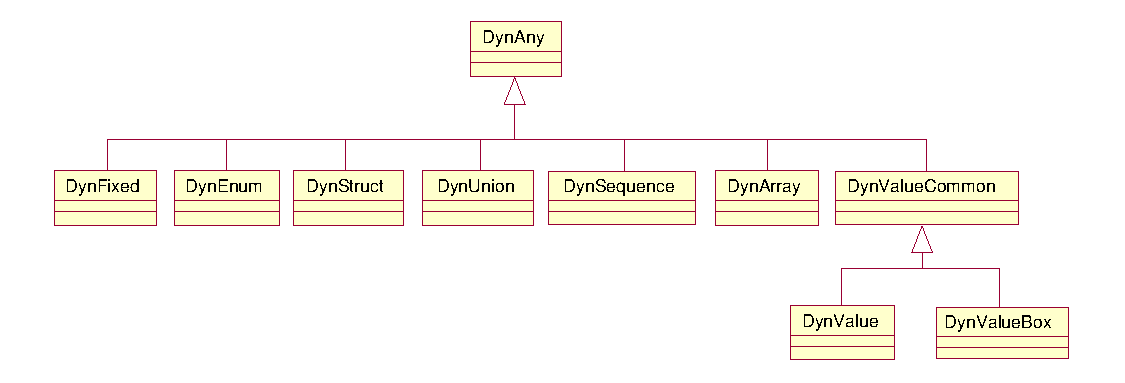
\includegraphics[width=\textwidth]{DynAny/dynany}
  \end{center}
\caption{DynAny Relationships}
\end{figure}


The DynAny interface is the base interface that represents values of
the basic types.  For each constructed type there is a corresponding
interface that extends the DynAny interface and defines operations
specific to the constructed type.  The table below lists the
interfaces in the DynamicAny module and the types they represent.


\begin{small}
\begin{longtable}{|p{6.3cm}|p{8.6cm}|}
\hline
~ \hfill \textbf {Interface} \hfill ~ & ~ \hfill \textbf {Type} \hfill ~ \endhead
\hline
\verb"DynAny" & \verb"basic types (boolean, long, etc.)" \\
\hline
\verb"DynFixed" & \verb"fixed" \\
\hline
\verb"DynEnum" & \verb"enum" \\
\hline
\verb"DynStruct" & \verb"struct" \\
\hline
\verb"DynUnion" & \verb"union" \\
\hline
\verb"DynSequence" & \verb"sequence" \\
\hline
\verb"DynArray" & \verb"array" \\
\hline
\verb"DynValue*" & \verb"non-boxed valuetype" \\
\hline
\verb"DynValueBox*" & \verb"boxed valuetype" \\
\hline

\end{longtable}
\end{small}

* Not currently implemented by JacORB.

\section{Usage Constraints}

Objects that implement interfaces in the DynamicAny module are
intended to be local to the process that constructs and uses them.
As a result, references to these objects cannot be exported to other
processes or externalized using ORB::object\_to\_string;  an
operation that attempts to do so will throw the MARSHAL system
exception.

\section{Creating a DynAny Object}

The DynAnyFactory interface is used to create a DynAny object.  There
are two operations for creating a DynAny object; these are listed in
the table below.


\begin{small}
\begin{longtable}{|p{6.3cm}|p{8.6cm}|}
\hline
~ \hfill \textbf {Operation} \hfill ~ & ~ \hfill \textbf {Description} \hfill ~ \endhead
\hline
\verb"create_dyn_any" & \verb"Constructs a DynAny object from an Any"
\verb"value" \\
\hline
\verb"create_dyn_any_from_ty"
\verb"pe_code" & \verb"Constructs a DynAny object from a"
\verb"TypeCode" \\
\hline

\end{longtable}
\end{small}

The example below illustrates how to obtain a reference to the
DynAnyFacory object and then use it to construct a DynAny object with
each of the create operations.  Exception handling is omitted for
brevity.

The following line of code imports the classes in the DynamicAny
package.

\begin{small}
\begin{verbatim}
import org.omg.DynamicAny.*;

\end{verbatim}
\end{small}

The following code segment obtains a reference to the DynAnyFacory
object.

\begin{small}
\begin{verbatim}
DynAnyFactory factory = null;
DynAny DynAny = null;
DynAny DynAny2 = null;
org.omg.CORBA.Any any = null;
org.omg.CORBA.TypeCode tc = null;
org.omg.CORBA.Object obj = null;

// obtain a reference to the DynAnyFactory
obj = orb.resolve_initial_references ("DynAnyFactory");

// narrow the reference to the correct type
factory = DynAnyFactoryHelper.narrow (obj);

\end{verbatim}
\end{small}

The following code segment creates a DynAny with each of the create
operations.

\begin{small}
\begin{verbatim}
// create a DynAny object from an Any
any = orb.create_any ();
any.insert_long (1);
DynAny = factory.create_dyn_any (any);

// create a DynAny object from a TypeCode
tc = orb.get_primitive_tc (org.omg.CORBA.TCKind.tk_long);
DynAny2 = factory.create_dyn_any_from_type_code (tc);

\end{verbatim}
\end{small}

If the Any value or TypeCode represents a constructed type then the
DynAny can be narrowed to the appropriate subtype, as illustrated
below.

The following IDL defines a struct type.

\begin{small}
\begin{verbatim}
// example struct type
struct StructType
{
   long field1;
   string field2;
};

\end{verbatim}
\end{small}

The following code segment illustrates the creation of a DynStruct
object that represents a value of type StructType.

\begin{small}
\begin{verbatim}
StructType type = null;
DynStruct dynStruct = null;

// create an Any that contains an object of type StructType
type = new StructType (999, "Hello");
any = orb.create_any ();
StructTypeHelper.insert (any, type);

// construct a DynAny from an Any and narrow it to a DynStruct
dynStruct = (DynStruct) factory.create_dyn_any (any);

\end{verbatim}
\end{small}

\section{Accessing the Value of a DynAny Object}

The DynAny interface defines a set of operations for accessing the
value of a basic type represented by a DynAny object.  The operation
to get a value of basic type $<$type$>$ from a DynAny has the form
get\_$<$type$>$.  The operation to insert a value of basic type
$<$type$>$ into a DynAny has the form insert\_$<$type$>$.  A
TypeMismatch exception is thrown if the type of the operation used to
get/insert a value into a DynAny object does not match the type of
the DynAny.

The operations for accessing the value of a constructed type
represented by a DynAny are defined in the interface specific to the
constructed type.  For example, the DynStruct interface defines the
operation get\_members, which returns a sequence of name/value pairs
representing the members of the struct or exception represented by a
DynStruct object.

\section{Traversing the Value of a DynAny Object}

DynAny objects can be viewed as an ordered collection of component
DynAnys.  For example, in a DynStruct object the ordered collection
of component DynAnys is the members of the struct or exception it
represents.  For DynAny objects representing basic types or
constructed types that do not have components, the collection of
component DynAnys is empty.

All DynAny objects have a current position.  For DynAnys representing
constructed types that have components, the current position is the
index of the component DynAny that would be obtained by a call to the
current\_component operation (described in the table below).  The
component DynAnys of a DynAny object are indexed from 0 to n-1, where
n is the number of components.  For DynAnys representing basic types,
or constructed types that do not have components, the current
position is fixed at the value -1.

The operations for traversing the component DynAnys of a DynAny
object are common to all DynAny subtypes, hence they are defined in
the DynAny base interface.  The table below lists the operations
available for traversing a DynAny object.


\begin{small}
\begin{longtable}{|p{6.3cm}|p{8.6cm}|}
\hline
~ \hfill \textbf {Operation} \hfill ~ & ~ \hfill \textbf {Description} \hfill ~ \endhead
\hline
\verb"seek" & \verb"Sets the current position to the"
\verb"specified index" \\
\hline
\verb"rewind" & \verb"Sets the current position to the first"
\verb"component (index 0)" \\
\hline
\verb"next" & \verb"Advances the current position to the"
\verb"next component" \\
\hline
\verb"component_count" & \verb"Returns the number of components" \\
\hline
\verb"current_component" & \verb"Returns the component at the current"
\verb"position" \\
\hline

\end{longtable}
\end{small}

The following code segment illustrates one way of traversing the
component DynAnys of a DynStruct object.  As the DynStruct is
traversed, the value of each component is obtained and printed.
Exception handling is omitted for brevity.

\begin{small}
\begin{verbatim}
DynAny curComp = null;

// print the value of the first component
curComp = dynStruct.current_component ();
System.out.println ("field1 = " + curComp.get_long ());

// advance to the next component
dynStruct.next ();

// print the value of the second component
curComp = dynStruct.current_component ();
System.out.println ("field2 = " + curComp.get_string ());

\end{verbatim}
\end{small}

The next code segment illustrates another way to perform the same
task.

\begin{small}
\begin{verbatim}
// go back to the first component
dynStruct.rewind ();  // same as calling seek (0)

// print the value of the first component
System.out.println ("field1 = " + dynStruct.get_long ());

// advance to the next component
dynStruct.seek (1);

// print the value of the second component
System.out.println ("field2 = " + dynStruct.get_string ());

\end{verbatim}
\end{small}

As the second code segment illustrates, if the component DynAny
represents a basic type, its value can be extracted (or inserted) by
calling the accessor operation on the parent DynAny directly, rather
than first obtaining the component using the current\_component
operation.

\section{Constructed Types}

This section describes the interfaces in the DynamicAny module that
represent the constructed types supported by JacORB.  Each of these
interfaces extends the DynAny interface.



\subsection{DynFixed}

A DynFixed object represents a fixed value.  Since IDL does not have
a generic type to represent a fixed type, the operations in this
interface use the IDL string type.  The value represented by a
DynFixed object can be accessed (as a string) using the get\_value
and set\_value operations.

A DynFixed object has no components.

\subsection{DynEnum}

A DynEnum object represents a single enumerated value.  The integer
(ordinal) value of the enumerated value can be accessed with the
get\_as\_ulong and set\_as\_ulong operations.  The string (IDL
identifier) value of the enumerated value can be accessed with the
get\_as\_string and set\_as\_string operations.

A DynEnum object has no components.

\subsection{DynStruct}

A DynStruct object represents a struct value or an exception value.
The current\_member\_name and current\_member\_kind operations return
the name and TCKind value of the TypeCode of the member at the
current position of the DynStruct.  The members of the DynStruct can
be accessed with the get\_members and set\_members operations.

The component DynAnys of a DynStruct object are the members of the
struct or exception.  A DynStruct representing an empty exception has
no components.

\subsection{DynUnion}

A DynUnion object represents a union value.  The value of the
discriminator can be accessed using the get\_discriminator and
set\_discriminator operations.

If the discriminator is set to a value that names a member of the
union then that member becomes active.  Otherwise, if the value of
the discriminator does not name a member of the union then there is
no active member.

If there is an active member, the member operation returns its value
as a DynAny object, and the member\_name and member\_kind operations
return its name and the TCKind value of its TypeCode.  These
operations throw an InvalidValue exception if the union has no active
member.

A DynUnion object can have either one or two components.  The first
component is always the discriminator value.  The second component is
the value of the active member, if one exists.

\subsection{DynSequence}

A DynSequence object represents a sequence.  The length of the
sequence can be accessed using the get\_length and set\_length
operations.  The elements of the sequence can be accessed using the
get\_elements and set\_elements operations.

The component DynAnys of a DynSequence object are the elements of the
sequence.

\subsection{DynArray}

A DynArray object represents an array.  The elements of the array can
be accessed using the get\_elements and set\_elements operations.

The component DynAnys of a DynArray object are the elements of the
array.

\section{Converting between Any and DynAny Objects}

The DynAny interface defines operations for converting between Any
objects and DynAny objects.  The from\_any operation initialises the
value of a DynAny with the value of a specified Any.  A TypeMismatch
exception is thrown if the type of the Any does not match the type of
the DynAny.  The to\_any operation creates an Any from a DynAny.

As an example of how these operations might be useful, suppose one
wants to dynamically modify the contents of some constructed type,
such as a struct, which is represented as an Any.  The following
steps will accomplish this task:

\begin{enumerate}
  \item  A DynStruct object is constructed from the TypeCode of the struct using the DynAnyFactory::create\_dyn\_any\_from\_type\_code operation.
  \item  The DynAny::from\_any operation is used to initialise the value of the DynStruct with the value of the Any.
  \item  The contents of the DynStruct can now be traversed and modified.
  \item  A new Any can be created to represent the modified struct using the DynAny::to\_any operation.
\end{enumerate}

\section{Further Examples}

The demo/dynany directory of the JacORB repository contains example
code illustrating the use of DynAny objects.  Further code can be
found in the org.jacorb.test.orb.dynany package of the JacORB-Test
repository.


%%% Local Variables: 
%%% mode: latex
%%% TeX-master: "../ProgrammingGuide"
%%% End: 
